\documentclass[tikz,border=12pt]{standalone}
\usepackage[T1]{fontenc}
\usepackage{mathpazo}
\usepackage{amsmath,amssymb}
\usetikzlibrary{arrows.meta, positioning, calc}

\definecolor{stblue}{HTML}{7B97AD}
\definecolor{rwgold}{HTML}{B8995E}
\definecolor{sage}{HTML}{7A9A7E}
\definecolor{dkbrown}{HTML}{3D3530}
\definecolor{wmgray}{HTML}{7B7067}
\definecolor{cream}{HTML}{F9F6F0}
\definecolor{border}{HTML}{D4C9B8}
\definecolor{terracotta}{HTML}{C47A6A}
\definecolor{lavender}{HTML}{907EA0}

\begin{document}
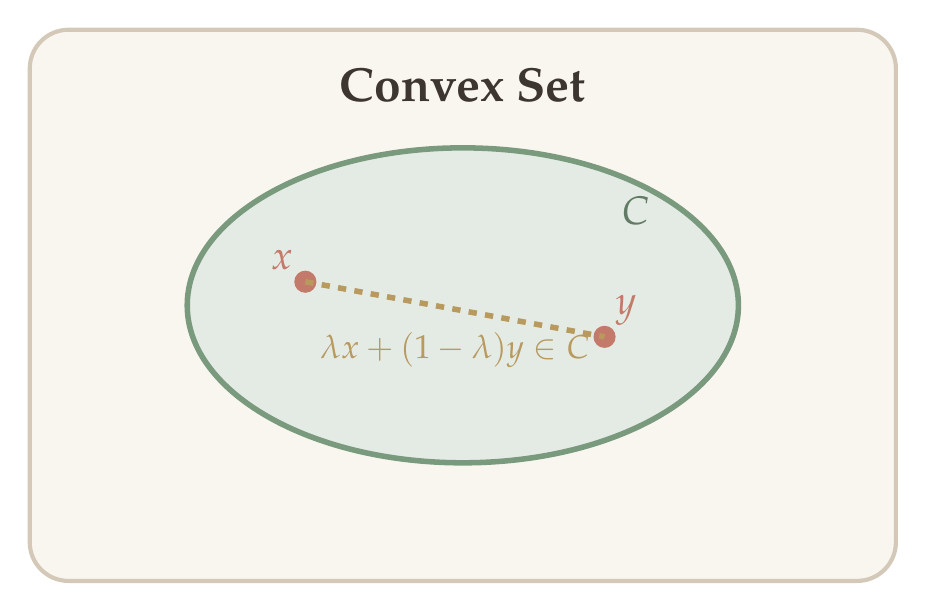
\begin{tikzpicture}[>={Stealth[length=4mm, width=3mm]}]

% Background
\fill[cream, rounded corners=14pt] (-0.5,-0.5) rectangle (10.5,6.5);
\draw[border, line width=1.5pt, rounded corners=14pt] (-0.5,-0.5) rectangle (10.5,6.5);

% Title
\node[text=dkbrown, font=\LARGE\bfseries] at (5,5.8) {Convex Set};

% Elliptical convex set
\fill[sage!20] (5,3) ellipse (3.5cm and 2.0cm);
\draw[sage, line width=2pt] (5,3) ellipse (3.5cm and 2.0cm);

% Label C
\node[text=sage!80!black, font=\Large\bfseries] at (7.2,4.2) {$C$};

% Points x and y
\coordinate (px) at (3.0,3.3);
\coordinate (py) at (6.8,2.6);

\fill[terracotta] (px) circle (4pt);
\fill[terracotta] (py) circle (4pt);

% Dashed line segment
\draw[rwgold, line width=2pt, dashed] (px) -- (py);

% Labels
\node[text=terracotta, font=\Large\bfseries, above left=1pt] at (px) {$x$};
\node[text=terracotta, font=\Large\bfseries, above right=1pt] at (py) {$y$};

% Midpoint label
\coordinate (mid) at ($(px)!0.5!(py)$);
\node[text=rwgold, font=\large, below=5pt] at (mid) {$\lambda x + (1-\lambda)y \in C$};

\end{tikzpicture}
\end{document}
